\documentclass[10pt]{exam}
\usepackage[hon]{template-for-exam}
\usepackage{tikz,multicol,cclicenses,hyperref}
\usetikzlibrary{shadings,shadows,arrows.meta,shapes.geometric}


\title{Angular Momentum}
\author{Rohrbach}
\date{\today}

\begin{document}
\maketitle


\section*{Quantities}

\renewcommand{\arraystretch}{2}

\begin{tabular}{p{9em}ccp{6.5em}}
  Concept & Linear/Translational Quantity & Angular/Rotational Quantity & \hfill ``Bridge'' \\ \hline\hline
  momentum \\[1em] & units: & units:  \\\hline
\end{tabular}

\vspace{10em}

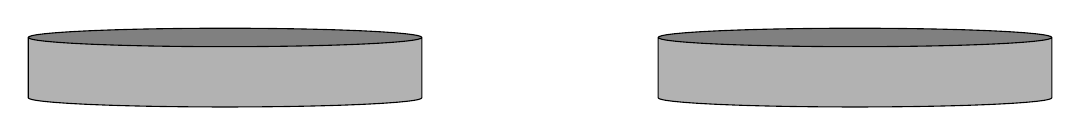
\begin{tikzpicture}
  \node[
    cylinder, 
    draw=black, 
    shape border rotate=90,
    minimum width=5cm,
    minimum height = 1cm,
    cylinder uses custom fill,
    cylinder body fill = gray!60,
    cylinder end fill = gray,
    anchor=center
    ] at (0,0) {};
  
    \node[
      cylinder, 
      draw=black, 
      shape border rotate=90,
      minimum width=5cm,
      minimum height = 1cm,
      cylinder uses custom fill,
      cylinder body fill = gray!60,
      cylinder end fill = gray,
      anchor=center
      ] at (8,0) {};
    
\end{tikzpicture}

\pagebreak

\section*{Practice}

\begin{questions}

\question
  An ice skater is spinning with her arms extended. She has a moment of inertia of 4.1~kg~m$^2$ and an initial angular velocity of 2.0~rad/s. She then pulls her arms in, reducing her moment of inertia to 1.5~kg~m$^2$.

  \begin{parts}
    \part 
      What is her new angular velocity after pulling her arms in?
    \part
      Calculate her initial and final rotational kinetic energy. Has her rotational kinetic energy increased or decreased? If so, explain why.
  \end{parts}
  \vs

\question
  The bicycle wheel is essentially a hoop of mass 8~kg and radius 0.4~m.  The turntable is essentially a disc of mass 5~kg and radius 0.5~m.  The instructor is essentially a particle located at the center of the axis.  If the bicycle wheel has an initial angular speed of 4.3 rad/s, what is the rate of rotation of the instructor and turntable after the wheel is flipped?
  \vs



  
\end{questions}



\end{document}